\chapter{Cwiczenie 3 - czwórnik RC}

\section{Polecenie}

Należało przekonstruować układ \textbf{CR} na czwórnik \textbf{RC}. Następnie zmierzyć charakterystyka amplitudową i fazową.
Na podstawie zmierzonych wartości należało wyznaczyć górną częstotliwość graniczną oraz porównać z wyliczoną wartością teoretyczną.

\section{Montaż układu}

Zmontowano układ używając opornika R2 = \textbf{3,9k}$\boldsymbol{\Omega}$, analogicznie do wcześniej zbudowanego układu CR używając trójnika rozdzielono sygnał, tak aby obserwować sygnał wejściowy oraz wyjściowy:
    \begin{figure}[h]
        \centering
        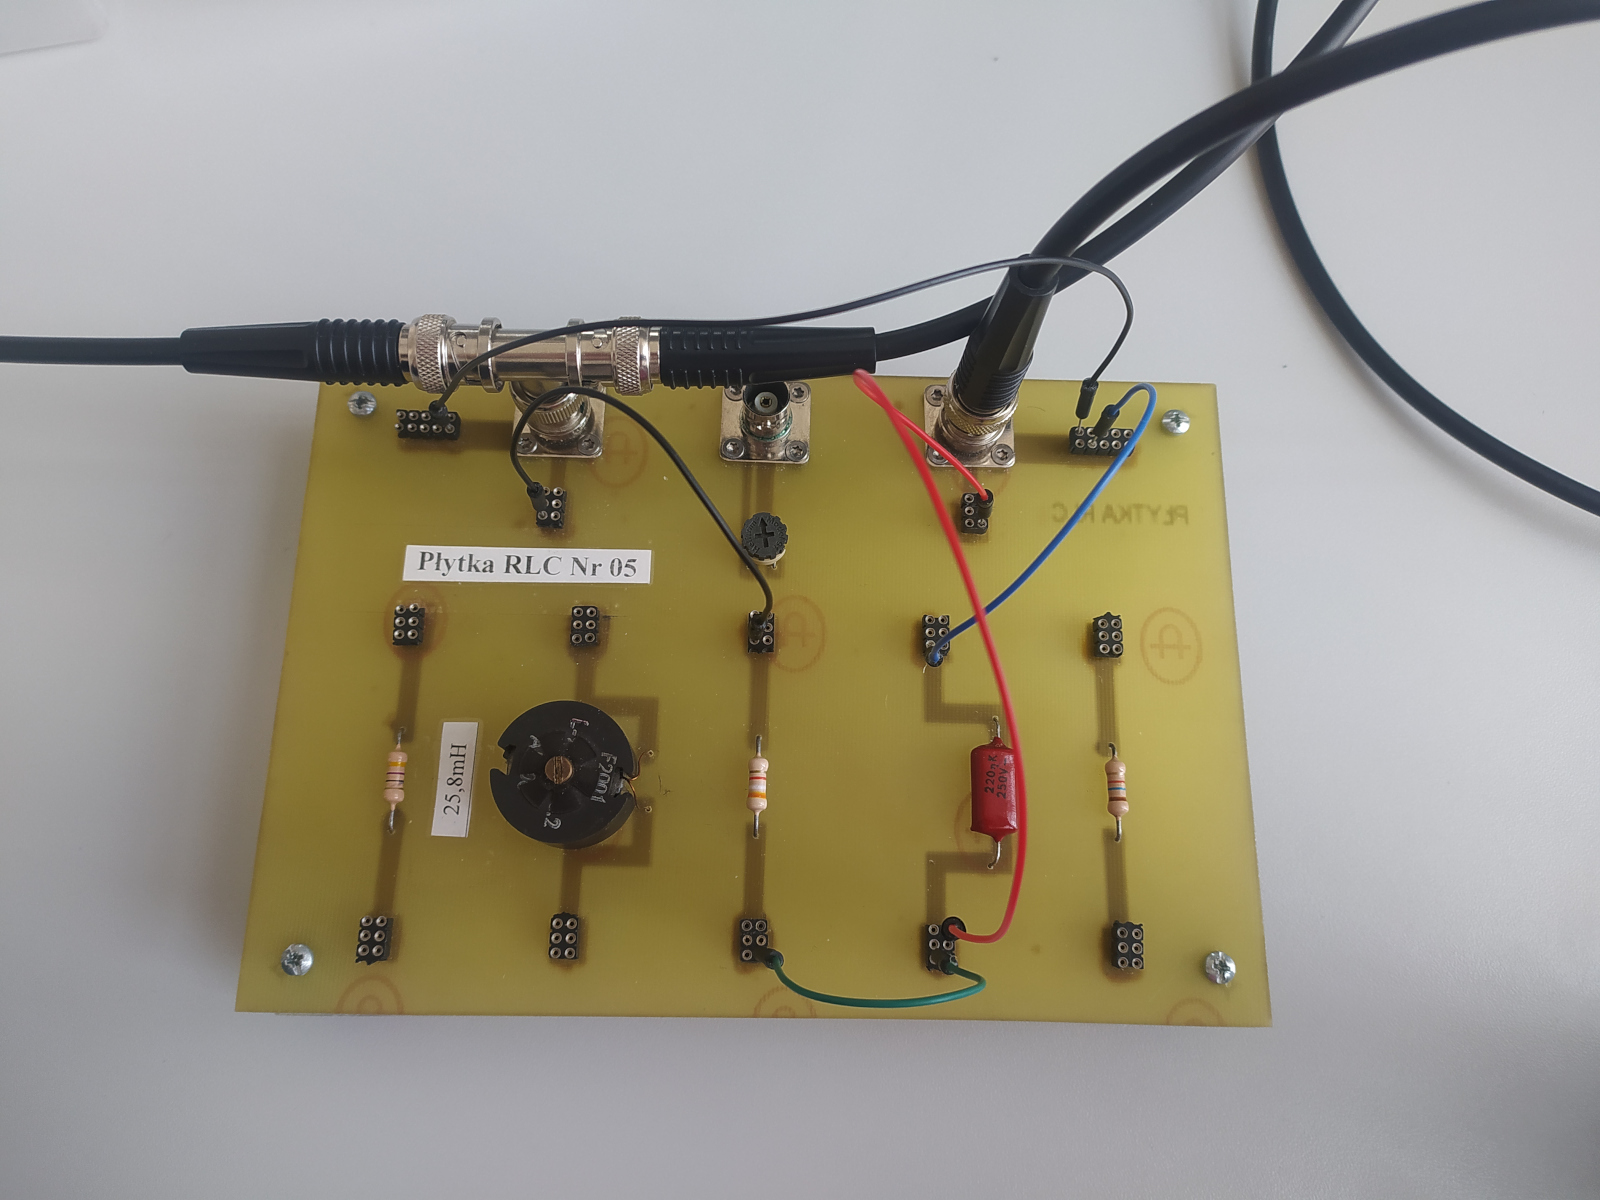
\includegraphics[scale=0.13]{img_phone/IMG_20220330_110044_smaller.jpg}
        \caption{Zmontowany czwórnik RC}
        \label{fig:built_RC}
    \end{figure}
    
\section{Badanie charakterystyk częstotliwościowych}
    Przystąpiono do badania charakterystyk częstotliwościowych.
    Przesyłano sygnał o amplitudzie \textbf{2V} oraz częstotliwościach z przedziału, pomiary pobierane zostały za pomocą funkcji wbudowanych w oscyloskopie. \textbf{1 kanał - wejście}, \textbf{2 kanał - wyjście}.

\pagebreak

\begin{itemize}
    \item \textcolor{purple}{Zmierzone wartości w postaci tabeli}:
\end{itemize}

\begin{center}
    \Large %tabelka Uwe Uwy phi
    \label{poprawa:pomiary_RC}
    \begin{tabular}{|>{\columncolor[gray]{0.8}}c|>{\columncolor[gray]{0.8}}c|c|>{\columncolor[gray]{0.8}}c|c|}
         \hline
         $f$ [Hz] & $U_{we}$ [V] & $U_{wy}$ [V] & $\frac{U_{wy}}{U_{we}}$ &  $\phi$ [$\degree$] \\
         \hline
         32.24 & 2 & 1.95 & 0.975 &  9.54 \\
         \hline
         50.03 & 1.99 & 1.91 & 0.96 & 14.24 \\
         \hline
         99.77 & 1.98 & 1.73 & 0.873 & 28.39 \\
         \hline
         200 & 1.98 & 1.34 & 0.67 & 46.09 \\
         \hline
         300.1 & 1.97 & 1.04 & 0.53 & 56.27 \\
         \hline
         418.6 & 1.96 & 0.848 & 0.432 & 64.29 \\
         \hline
         503.1 & 1.96 & 0.688 & 0.351 & 68.51 \\
         \hline
         682.6 & 1.96 & 0.525 & 0.268 & 74.15 \\
         \hline
         700 & 1.96 & 0.510 & 0.26 & 74.47 \\
         \hline
         857 & 1.96 & 0.429 & 0.219 & 77.05 \\
         \hline
         899 & 1.96 & 0.405 & 0.206 & 77.33 \\
         \hline
         1000 & 1.96 & 0.368 & 0.188 & 78.75 \\
         \hline
    \end{tabular}
\end{center}

%osciloscope_figures 
{ 
\begin{figure}[H]
    \centering
    \begin{subfigure}[h]{0.4\textwidth}
        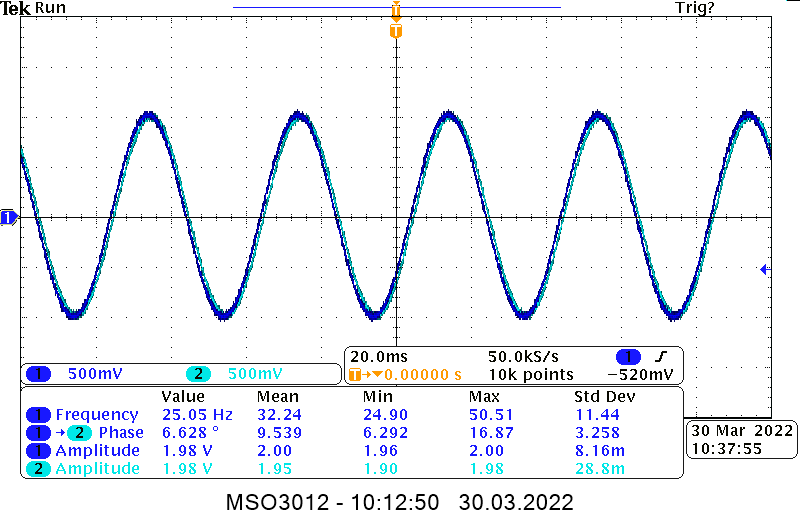
\includegraphics[width=\textwidth]{img_osciloscope/RC/RC_25Hz_cropped.png}
        \caption*{25Hz}
    \end{subfigure}
    \begin{subfigure}[h]{0.4\textwidth}
        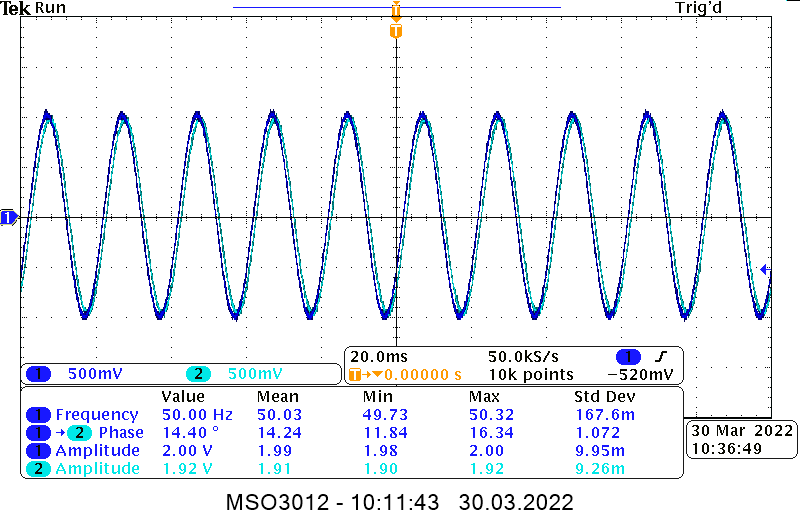
\includegraphics[width=\textwidth]{img_osciloscope/RC/RC_50Hz_cropped.png}
        \caption*{50Hz}
    \end{subfigure}
\end{figure}

\begin{figure}[H]
    \centering    
    \begin{subfigure}[h]{0.4\textwidth}
        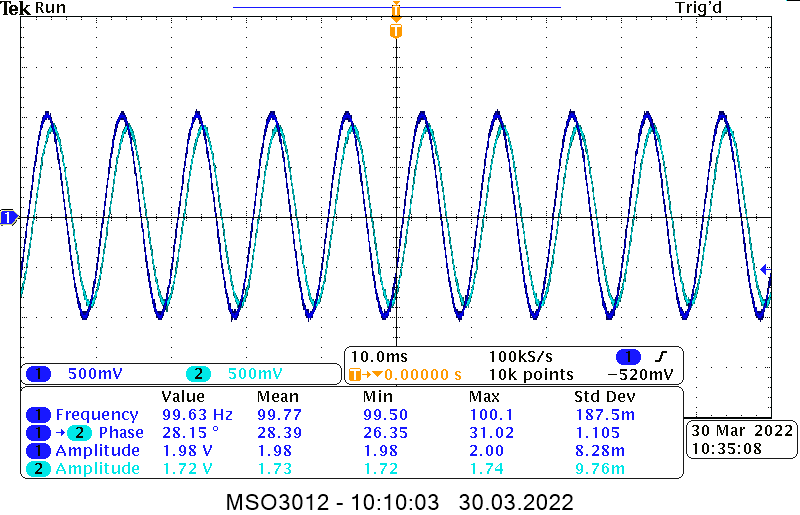
\includegraphics[width=\textwidth]{img_osciloscope/RC/RC_100Hz_cropped.png}
        \caption*{100Hz}
    \end{subfigure}
    \begin{subfigure}[h]{0.4\textwidth}
        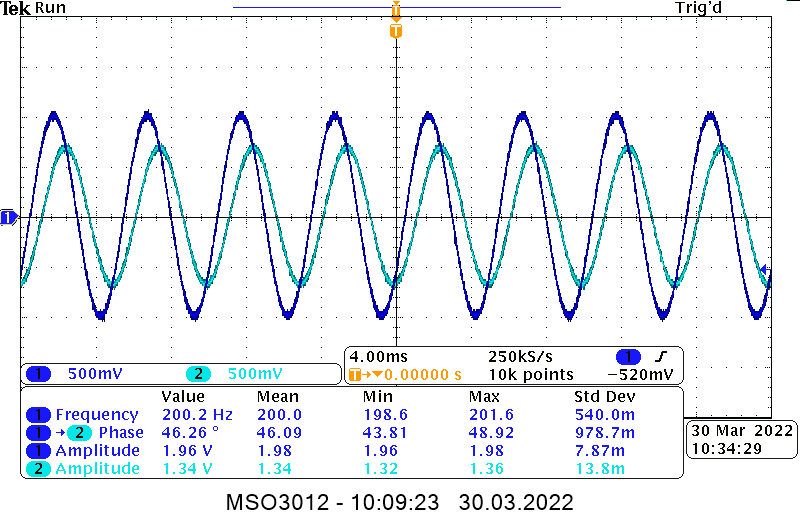
\includegraphics[width=\textwidth]{img_osciloscope/RC/RC_200Hz_cropped.png}
        \caption*{200Hz}
    \end{subfigure}
\end{figure}

\begin{figure}[H]
    \centering
    \begin{subfigure}[h]{0.4\textwidth}
        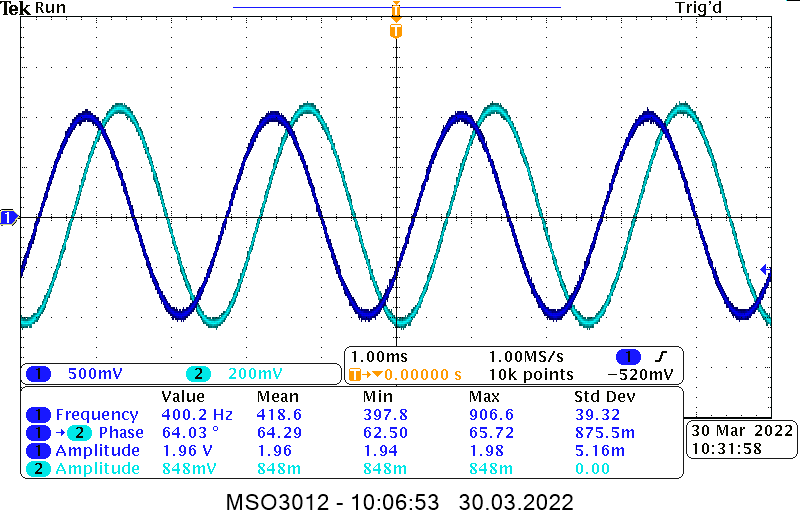
\includegraphics[width=\textwidth]{img_osciloscope/RC/RC_400Hz_cropped.png}
        \caption*{400Hz}
    \end{subfigure}
    \begin{subfigure}[h]{0.4\textwidth}
        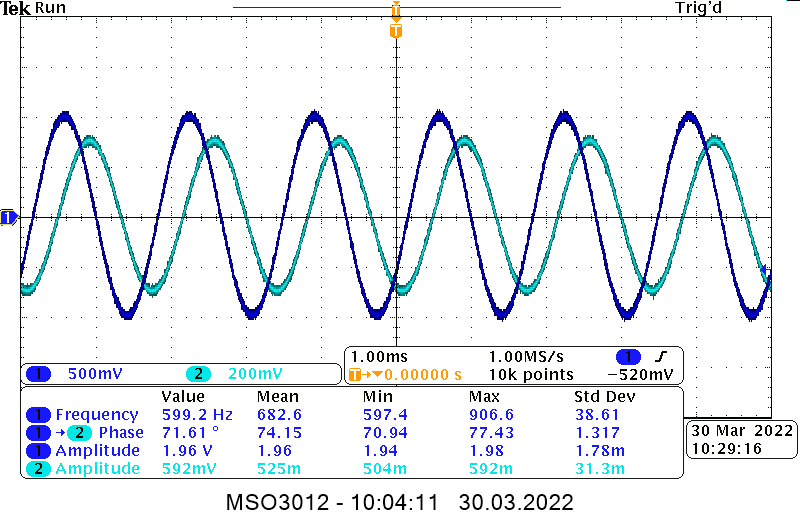
\includegraphics[width=\textwidth]{img_osciloscope/RC/RC_600Hz_cropped.png}
        \caption*{600Hz}
    \end{subfigure}
\end{figure}

\begin{figure}[H]
    \centering
    \begin{subfigure}[h]{0.4\textwidth}
        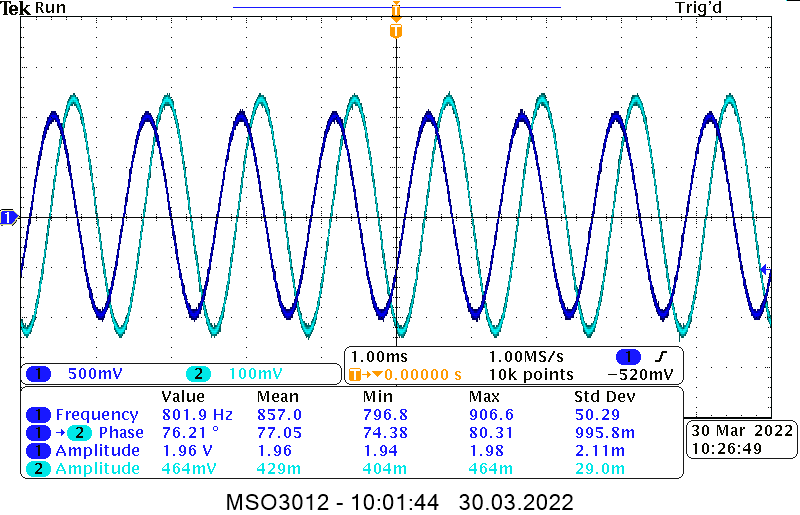
\includegraphics[width=\textwidth]{img_osciloscope/RC/RC_800Hz_cropped.png}
        \caption*{800Hz}
    \end{subfigure}
    \begin{subfigure}[h]{0.4\textwidth}
        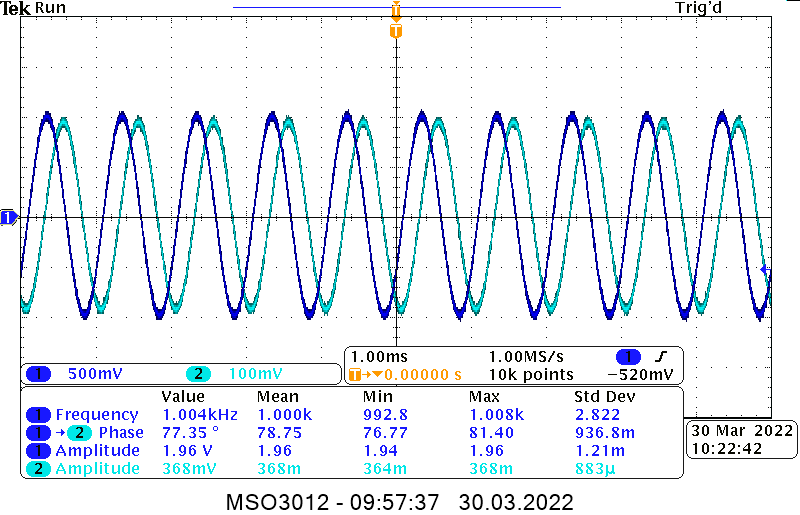
\includegraphics[width=\textwidth]{img_osciloscope/RC/RC_1000Hz_cropped.png}
        \caption*{10000Hz}
    \end{subfigure}
\end{figure}
}

\section{Charakterystyka amplitudowa}
    \begin{itemize}
        \item Stałe:
            \begin{gather}
                \tau = RC = 0.8 * 10^{-3}s \\
                \omega_0 = \frac{1}{RC} = \frac{1}{\tau}
            \end{gather}
        \item Funkcja przejścia:
            \begin{equation}
                T(\omega) = \frac{Z_2}{Z_1+Z_2} = \frac{\frac{1}{j \omega C}}{{R + \frac{1}{j \omega C}}} = \frac{1}{1 + j \omega RC} = \frac{1}{1 + j \frac{\omega}{\omega_0}}
                \label{eqn:f_przejscia_RC}
            \end{equation}
        \item Charakterystyka amplitudowa:
            \begin{equation}
                |T(\omega)| = \sqrt{\frac{1}{1 + (\frac{\omega}{\omega_0})^2}}
                \label{eqn:char_amp_RC}
            \end{equation}
        \item Górna częstotliwość graniczna teoretyczna wyniosła:
            \begin{equation}
                f_t = \frac{1}{2 \pi \tau} \approx \textbf{198.94Hz}
            \end{equation}
        \item Górna częstotliwość graniczna eksperymentalna wyniosła:
            \begin{equation}
                f_e \approx \textbf{180,5Hz}
            \end{equation}
        \item Różnica między wartością eksperymentalną a teoretyczną wyniosła $\boldsymbol{\Delta}$ = \textbf{18.44Hz}\\
        Funkcja zgadza się z teoretyczną. \\
        Pomiar został uznany za poprawny.
        \begin{figure}[H]
            \centering
            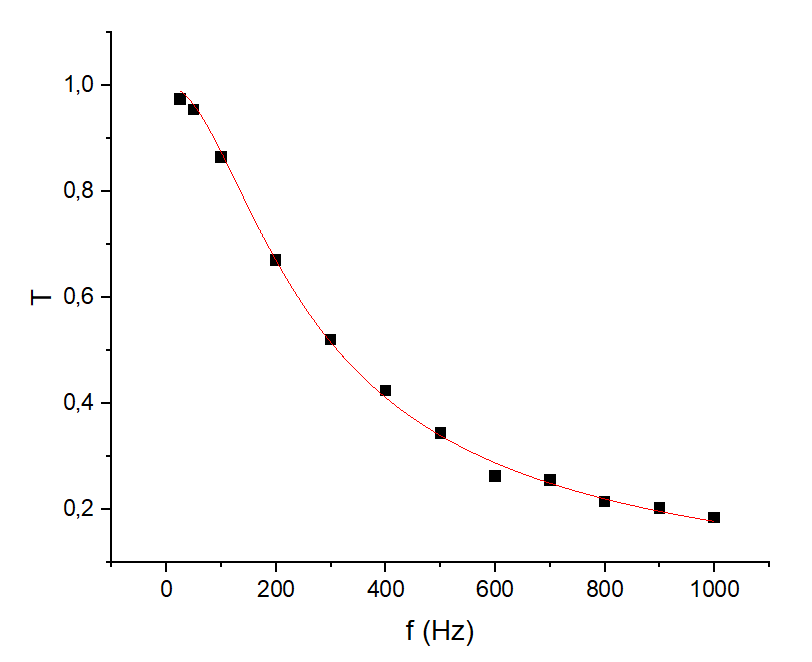
\includegraphics[scale=0.55]{img_wykresy/amplitudowa_RC.png}
            \caption{Charakterystyka amplitudowa | $\blacksquare$ - punkty eksperymentalne}
            \label{fig:CR_amp}
        \end{figure}
    \end{itemize}

\section{Charakterystyka fazowa}

\begin{itemize}
    \item Stałe:
        \begin{gather}
            \tau = RC = 0.8 * 10^{-3}s \\
            \omega_0 = \frac{1}{RC} = \frac{1}{\tau}
        \end{gather}
    \item Funkcja przejścia wynosi:
        \begin{equation}
            T(\omega) = \frac{1 - j \frac{\omega}{\omega_0}}{1 + (\frac{\omega}{\omega_0})^2}
        \end{equation}
    \item Charakterystyka fazowa:
        \begin{equation}
            \phi(\omega) = \arctan({\frac{Im T(\omega)}{Re T(\omega)}}) = -\arctan({\frac{\omega}{\omega_0}})
        \end{equation}
    \item Górna częstotliwość graniczna teoretyczna wyniosła: 
        \begin{equation}
            f_t = \frac{1}{2 \pi \tau} \approx \textbf{198.94Hz}
        \end{equation}
    \item Górna częstotliwość graniczna eksperymentalna wyniosła:
        \begin{equation}
            f_e \approx 191,35Hz
        \end{equation}
    \item Różnica między wartością eksperymentalną a teoretyczną wyniosła $\boldsymbol{\Delta}$ = \textbf{7.59Hz}\\
        Funkcja zgadza się z teoretyczną. \\
        Pomiar został uznany za poprawny.
    \begin{figure}[H]
        \centering
        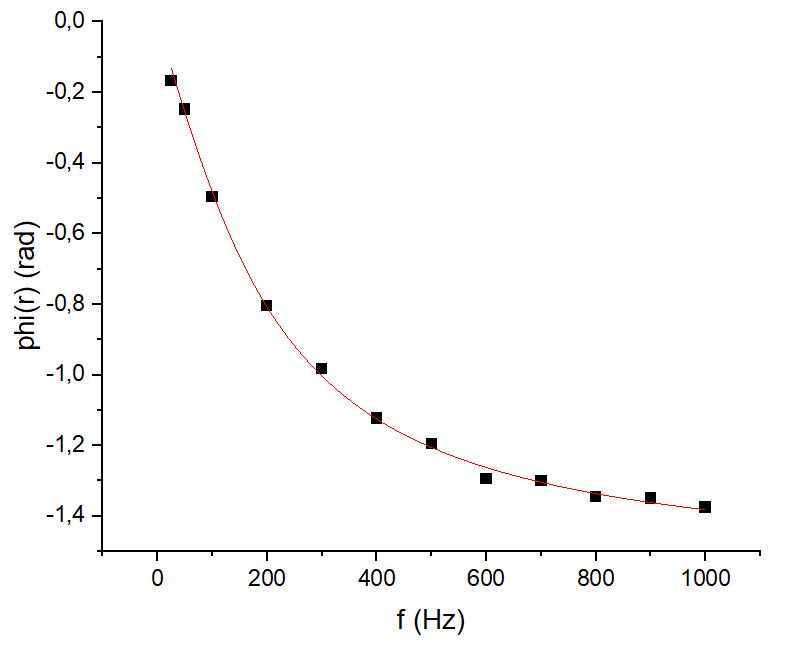
\includegraphics[scale=0.55]{img_wykresy/fazowa_RC.png}
        \caption{Charakterystyka fazowa | $\blacksquare$ - punkty eksperymentalne}
        \label{fig:CR_amp}
    \end{figure}
\end{itemize}


\section{Sygnał prostokątny}

Podobnie jak w ćwiczeniu 2, należało zaobserwować przebieg impulsów prostokątnych podawanych z różnym okresem \langle\textbf{0.5}$\boldsymbol{\tau}$ - \textbf{10}$\boldsymbol{\tau}$\rangle

\label{poprawa:dodanie_wartosci_okresow_4_6}

\begin{figure}[H]
    \centering
    \begin{subfigure}[h]{0.45\textwidth}
        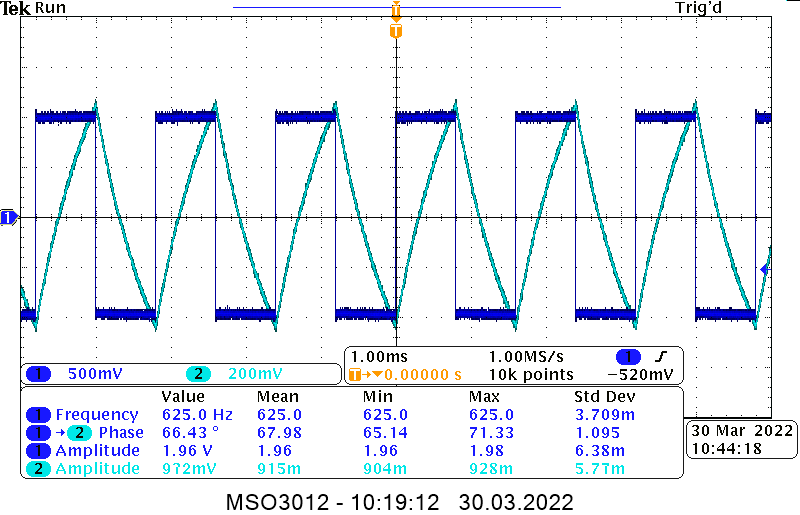
\includegraphics[width=\textwidth]{img_osciloscope/RC_pros/RC_prostokat_0_5_tau_cropped.png}
        \caption*{0.5$\tau$ = 625Hz}
    \end{subfigure}
    \begin{subfigure}[h]{0.45\textwidth}
        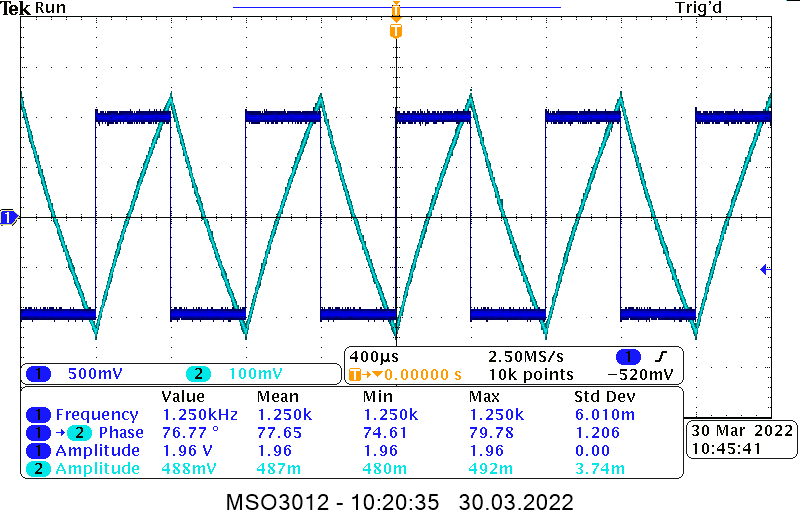
\includegraphics[width=\textwidth]{img_osciloscope/RC_pros/RC_prostokat_1_0_tau_cropped.png}
        \caption*{1.0$\tau$ = 1.25kHz}
    \end{subfigure}
\end{figure}

\begin{figure}[H]
    \centering
    \begin{subfigure}[h]{0.45\textwidth}
        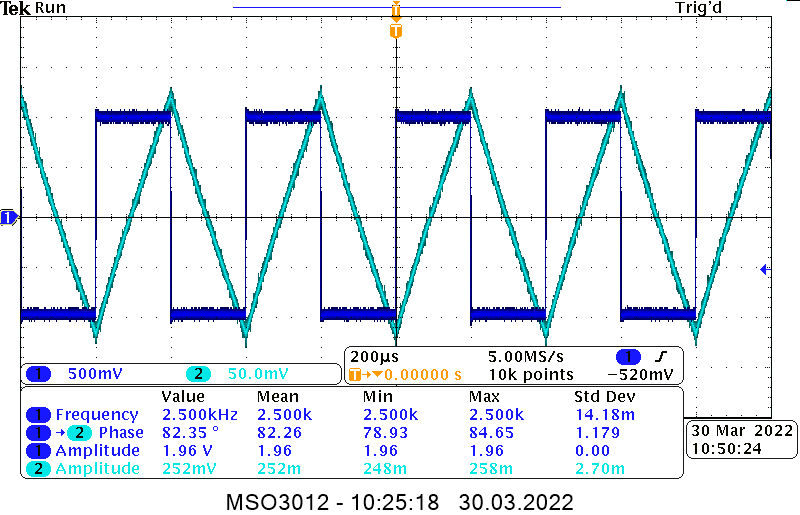
\includegraphics[width=\textwidth]{img_osciloscope/RC_pros/RC_prostokat_2_0_tau_cropped.png}
        \caption*{2.0$\tau$ = 2.5kHz}
    \end{subfigure}
    \begin{subfigure}[h]{0.45\textwidth}
        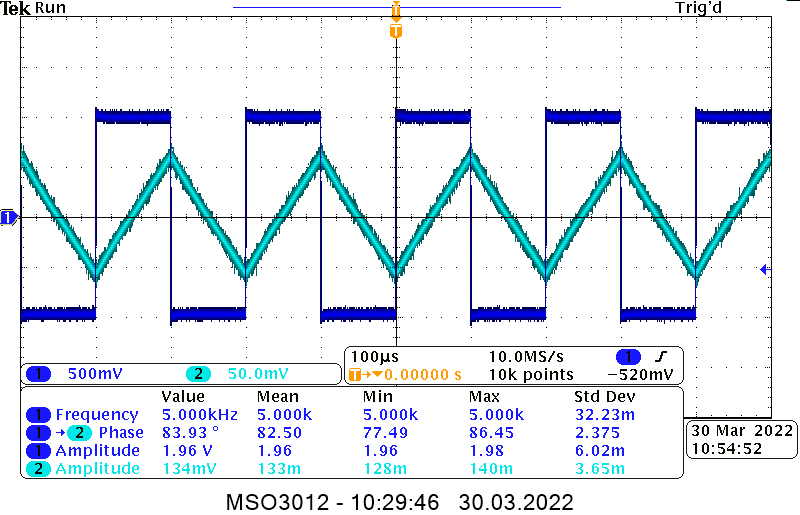
\includegraphics[width=\textwidth]{img_osciloscope/RC_pros/RC_prostokat_4_0_tau_cropped.png}
        \caption*{4.0$\tau$ = 5kHz}
    \end{subfigure}
\end{figure}

\begin{figure}[H]
    \centering
    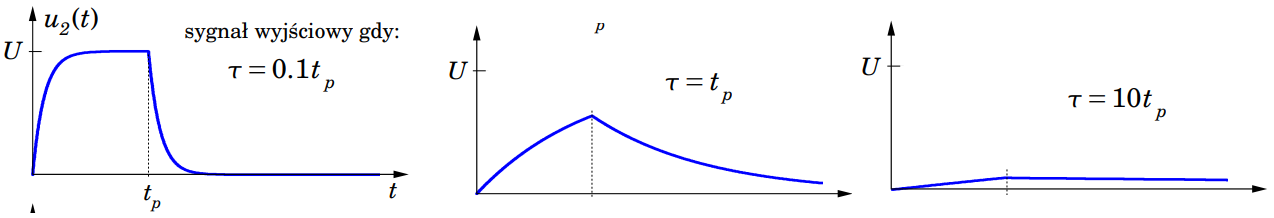
\includegraphics[width=\textwidth]{img_wyklad/teor_pros_RC.png}
    \caption{Teoretyczne wykresy prostokątnych sygnałów przechodzących przez układ RC}
    \label{fig:my_label}
\end{figure}

\begin{itemize}
    \item Nie zaobserwowano przejścia fali prostokątnej przez układ gdy \textbf{T = 0.1}\boldsymbol{\tau}.
    \item Pozostałe wykresy zgadzają się z teoretycznymi przewidywaniami.
    \item Poczynając od \approx T = 4$\tau$ sygnał wyjściowy jest w pełni poprawnie scałkowany.
\end{itemize}
